\begin{frame}{Workflow: History}
\footnotesize

\onslide<2->{
\begin{block}{Inspect history}
\begin{semiverbatim}
\$ git log

\$ git log --oneline
%\only<3->{
%Noch keine Commits
%
%Unversionierte Dateien:
%  (benutzen Sie "git add <Datei>...", um die Änderungen zum Commit vorzumerken)
%	file.txt
%
%nichts zum Commit vorgemerkt, aber es gibt unversionierte Dateien
%(benutzen Sie git add zum Versionieren)
%}
\end{semiverbatim}
\end{block}
}

\begin{center}
\only<3>{
 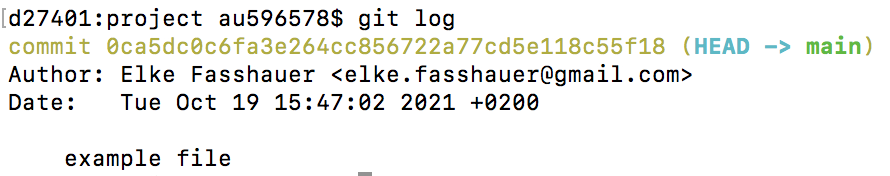
\includegraphics[width=0.8\textwidth]{pics/git_log.png}
}
\end{center}

\end{frame}
